\documentclass[spanish,notes=hide]{beamer}

%To create 'handout' version (Copyright: Diego Berrueta)
%\documentclass[handout,notes=show]{beamer}

\usetheme{Marburg}
%\usepackage{beamerthemesplit}

\usepackage[spanish]{babel}
\usepackage[utf8]{inputenc}
\usepackage{listings}
\usepackage{graphicx}
\usepackage{colortbl}
\usepackage{array}
\usepackage{eurosym}

\title{Mailing lists meet the Semantic Web}
\author{
Sergio Fern\'andez\inst{1} 
\and
\textbf{Diego Berrueta}\inst{1} 
\and
Jose E. Labra\inst{2}
}
\institute{%
Fundaci\'on CTIC, \\
Gij\'on, Asturias, Spain,\\
\email{\{sergio.fernandez,diego.berrueta\}@fundacionctic.org} %FIXME
\and
Universidad de Oviedo,\\
Computer Science Department,\\
Oviedo, Asturias, Spain,\\
\email{labra@uniovi.es}\\
}
\date{27 April 2007}

\begin{document}


%tableofcontents

%\AtBeginSection[]
%{
%   \begin{frame}
%       \frametitle{Tabla de contenidos}
%       \tableofcontents[currentsection]
%   \end{frame}
%}

%\AtBeginSubsection[] 
%{
%   \begin{frame}
%       \frametitle{Tabla de contenidos}
%       \tableofcontents[currentsection,currentsubsection]
%   \end{frame}
%}

%listings

\definecolor{darkred}{rgb}{0.5, 0, 0}
\definecolor{violet}{rgb}{1, 0, 1}
\definecolor{green}{rgb}{0.3, 0.95, 0.3}
\definecolor{listinggray}{gray}{0.97}

\lstset{
	basewidth=0.50em,
	backgroundcolor=\color{listinggray},
	basicstyle=\footnotesize\ttfamily,
	keywordstyle=\bfseries,
	stringstyle=\itshape,
	commentstyle=\itshape,
	showspaces=false,
	showtabs=false,
	showstringspaces=false,
	frame=trbl,
	extendedchars=true,
	numbers=none,
	aboveskip=0.5cm,
	belowskip=0.5cm,
	xleftmargin=0cm,
	xrightmargin=0cm
}

\lstdefinelanguage{mbox}{%no funciona!
	morekeywords = {From, Message, Date, Organization, To, Subject }
}

\lstdefinelanguage{SPARQL}{%
	morekeywords = {PREFIX, SELECT, DISTINCT, WHERE }
}


\maketitle

\section{Introduction}
\frame
{
  \frametitle{Introduction}

  \begin{itemize}
   \item<2-> \begin{large}\textbf{Actual situation:}\end{large}
	\begin{itemize}
	  \item \begin{large}Miles de listas de correo\end{large}
	  \item \begin{large}Publicación en HTML\end{large}
	\end{itemize}
   \vspace{0.8cm}
   \item<3-> \textbf{Problems:}
	\begin{itemize}
	  \item \begin{large}Pérdida de información\end{large}
	  \item \begin{large}Marcado estructurado sin valor semántico\end{large}
	  \item \begin{large}Problemas en las búsquedas tradicionales\end{large}
	\end{itemize}
  \end{itemize}
}

\section{SIOC}
\frame{
  \frametitle{SIOC Ontology}

  FIXME
}
\frame{
  \frametitle{Extending SIOC Ontology}

  FIXME
}

\section{Software tools}
\frame
{
  \frametitle{Software tools}

  \begin{columns}
   \begin{column}{0.35\textwidth}
	El proyecto SWAML se compone de varias partes:
	\begin{itemize}
	 \item \begin{Large}SWAML\end{Large}
	 \item \begin{Large}Buxon\end{Large}
	\end{itemize}
   \end{column}
   \begin{column}{0.65\textwidth}
	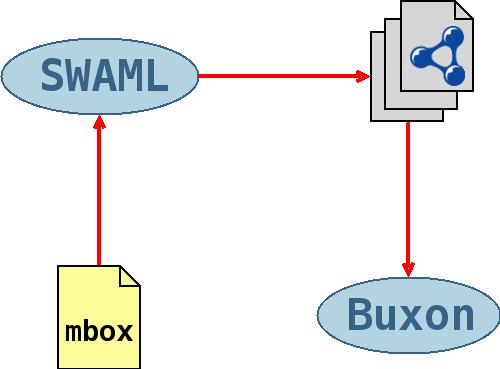
\includegraphics[width=0.95\textwidth]{images/componentes.png}
   \end{column}
  \end{columns}
}
\frame
{
  \frametitle{SWAML}

  \begin{columns}
   \begin{column}{0.5\textwidth}
	\begin{center}
	  \only<1>{
\includegraphics[width=0.95\textwidth]{images/swaml-0.png}}
	  \only<2>{
\includegraphics[width=0.95\textwidth]{images/swaml-1.png}}
	  \only<3>{
\includegraphics[width=0.95\textwidth]{images/swaml-2.png}}
	  \only<4>{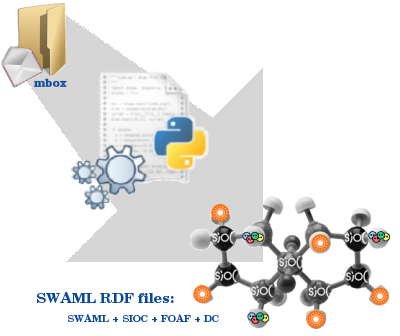
\includegraphics[width=0.95\textwidth]{images/swaml-3.png}}
	\end{center}
   \end{column}
   \begin{column}{0.5\textwidth}
	\begin{Large}batch process:\end{Large}
	\begin{enumerate}
	 \item<2-> mbox
	 \item<3-> parser
	 \item<4-> serialize to RDF/XML 
	\end{enumerate}
   \end{column}
  \end{columns}
}
\frame
{
  \frametitle{Buxon}

  \begin{columns}
   \begin{column}{0.32\textwidth}
	\begin{itemize}
	  \item a \texttt{sioc:Forum} browser
	  \item Recomposición de la lista de correo
	  \item Implementación más completa de SIOC
	\end{itemize}
   \end{column}
   \begin{column}{0.68\textwidth}
	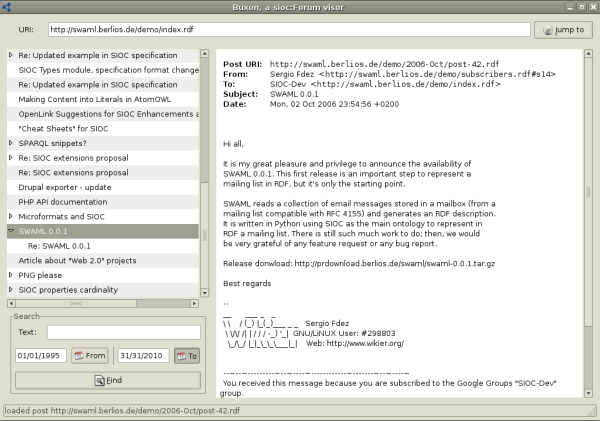
\includegraphics[width=\textwidth]{images/buxon.png}
   \end{column}
  \end{columns}
}

\section{Conclusions and future work}
\frame
{
  \frametitle{Conclusions}

  FIXME

}
\frame
{
  \frametitle{Future Work}

  \begin{itemize}
   \item \begin{Large}Acceder a cuentas de GMail\end{Large}
   \item \begin{Large}Marcado semántico para el cuerpo de los mensajes\end{Large}
   \item \begin{Large}API en Python para SIOC\end{Large}
   \item \begin{Large}Integración con Mailman\end{Large}
   \item \begin{Large}Paquete en Debian GNU/Linux\end{Large}
   \item \begin{Large}\textit{Submission} al W3C\end{Large}
  \end{itemize}
}

\section{Demostration}
\frame
{
  \frametitle{Practical demostration}

  \begin{center}
    \LARGE{\textbf{Let's go...}}
  \end{center}
}

\appendix

\section{More information}
\frame
{
  \begin{center}
    More information at the project Web page:\\
    \vspace{1cm}
    \LARGE{\href{http://swaml.berlios.de/}{http://swaml.berlios.de/}}\\
  \end{center}

}

\section{License}
\frame
{
  \begin{center}
    \LARGE{\textbf{Mailing lists meet\\the Semantic Web}}\\
    \vspace{1cm}
    \vspace{1cm}
    \begin{tiny}
	This talk is distributed under the terms of:\\
	\textbf{CreativeCommons license}\\
	
\includegraphics[width=3.5cm]{images/creativecommons.png}
    \end{tiny}
  \end{center}
}

\end{document}
